\section{Class diagram}

As you can see in the following class diagram of our current website implementation, it has once again changed significantly thanks to the addition of various small classes and the addition/modification of a few attribute. \newline

First a latitude and longitude attribute were added both to the player and court class. You can also notice that player is no linked to a ranking class which allows us to store ranking much more efficiently in the database. This can also been seen on the website as classement is now a drop down list rather than a simple text field.\newline

Many other small classes have been added to reduce string duplication in database such as TounoiTitle, TournoiCategorie and InfoTournoi. While InfoTounoi and TounoiTitle are mostly present to make our implementation more efficient in it's usage of memory space, The new TounoiCategorie class serve another purpose. Under the request of the client we modified our website handling of pair registration to automatically allocate newly registered pair to existing tournament, this class allowing us to store the automatic choice criteria.\newline

In reaction to the client's input, a new field was also created in the court class that allows us to register if that specific court was used in last year's tournament, this will allow staff to see year after year which court are more likely to be available for the tournament. \newline

The rest of the change involves the Pair and Arbre class, rather than storing the winner of a tournament in the arbre class as we did previously, it has been moved for efficiency to the Pair class, which now also records finalist for ease of display. A court attribute was also added to the arbre class, allowing us to record the court used for that knock-off tournament.

\begin{figure}[!ht]
	\centering
	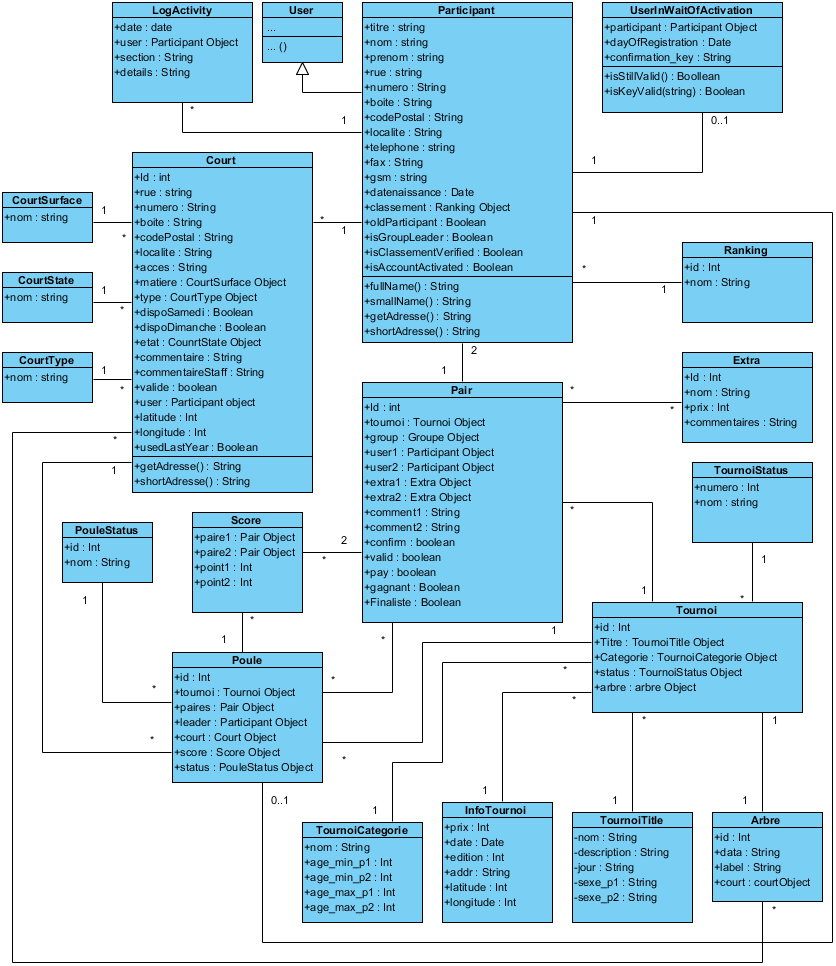
\includegraphics[width=1\linewidth]{class.png}
	\caption{Class diagram of our current implementation}
	\label{fig:length_eight_mouse}
\end{figure}
\FloatBarrier